{\section{Linear PDEs and Separation of Variables}
\subsection{Reminder of Superposition}

We will study \term{pure boundary value problems (BVP)}, which would be linear, of the form
\begin{subequations}
    \begin{align}
        P \psi\pqty{\vb{x}} = 0 &\qfor \vb{x} \in \Omega, \\
        \text{\term{Boundary Conditions}} &\qfor \vb{x} \in \partial \Omega.
    \end{align}
\end{subequations}

Instead, if we study an \term{initial BVP (BVP)}, then the equation be of the form
\begin{subequations}
    \begin{align}
        Q \phi\pqty{\vb{x}, t} = 0 &\qfor \pqty{\vb{x}, t} \in \Omega \times \oointv{0}{T}, \\
        \text{\term{Boundary Conditions}} &\qfor \pqty{\vb{x}, t} \in \partial \Omega \times \oointv{0}{T}, \\
        \text{\term{Initial Conditions}} &\qfor \pqty{\vb{x}, t} \in \Omega \times \Bqty{0}.
    \end{align}
\end{subequations}

Here, \(P, Q\) are linear partial differential operators, and \(\Omega \subset \RR^n\) will be open, bounded and connected. We work with \(n = 1, 2\) and 3.

Note the following observation. For an IBVP problem, we can break this up into simpler problems, splitting up the boundary and initial conditions:
\begin{subequations}
    \begin{align}
        Q \phi_1 \pqty{\vb{x}, t} = 0 &\qfor \pqty{\vb{x}, t}, \\
        \text{Boundary Conditions} = 0 &\qfor \pqty{\vb{x}, t} \in \partial \Omega \times \oointv{0}{T}, \\
        \text{Initial Conditions} &\qfor \pqty{\vb{x}, t} \in \Omega \times \Bqty{0}.
    \end{align}
\end{subequations}
and
\begin{subequations}
    \begin{align}
        Q \phi_2 \pqty{\vb{x}, t} = 0 &\qfor \pqty{\vb{x}, t}, \\
        \text{Boundary Conditions} &\qfor \pqty{\vb{x}, t} \in \partial \Omega \times \oointv{0}{T}, \\
        \text{Initial Conditions} = 0 &\qfor \pqty{\vb{x}, t} \in \Omega \times \Bqty{0}.
    \end{align}
\end{subequations}
then by linearity, the function \(\phi = \phi_1 + \phi_2\) solves our original IVBP.

Furthermore, observe that for problems in this section, it will turn out that \(\Omega\), possibly aftersome change of variables, will be come a line/rectangle/cuboid. Without loss of generality, we may assume that all boundary conditions vanish on all but one endpoint/edge/face.

\begin{example}
    Consider \(P \psi = 0\) for \(\pqty{x, y} \in \oointv{0}{1} \times \oointv{0}{1}\), with \(\psi = f_i\) on the \(i\)th side for the boundary conditions. Instead, using linearity, we consider \(\psi_i\) for \(i = 1, 2, 3, 4\) with the conditions
    \begin{subequations}
        \begin{align}
            P \psi_i = 0 &\qfor \pqty{x, y} \in \oointv{0}{1} \times \oointv{0}{1}, \\
            \psi_i = 0 &\qfor \text{side }\neq i, \\
            \psi_i = f_i &\qfor i\text{th side}.
        \end{align}
    \end{subequations}
    the note that \(\psi = \psi_1 + \psi_2 + \psi_3 + \psi_4\) solves the original problem.
\end{example}

Linearity is the best behaviour we have with such problems, and we should fully utilise this property.

\subsection{Laplace's Equation}

For a scalar function \(\functiondomain{\phi}{\RR^n}{\RR}\), Laplace's equation is equivalent to \(\laplacian 
\phi = 0\). For example, on \(\RR^3\) with Cartesian coordinates \(\pqty{x, y, z}\), the Cartesian Laplacian is given by
\begin{equation}
    \laplacian = \div \grad = \pdv[2]{x} + \pdv[2]{y} + \pdv[2]{z}.
\end{equation}

Intuitively, the Laplacian \(\laplacian \phi \pqty{\vb{x}}\) measures the extend to which \(\phi\pqty{\vb{x}}\) differs from its average over an infinitesimal ball centred at \(\vb{x}\). So if \(\laplacian \phi\pqty{\vb{x}} = 0\), then \(\phi\pqty{\vb{x}}\) agrees with its nearby averages (in the limit). This suggests that if a function satisfies the Laplace's equation, then there is a state of ``equilibrium'', and we say a function \(\phi\) being \term{harmonic} if \(\laplacian \phi\pqty{\vb{x}} = 0\).

\begin{example}
    Let the vector field \(\functiondomain{\vb{u}}{\RR^3}{\RR^3}\) denote the velocity fluid of some incompressible fluid (\(\div \vb{u} = 0\)). Suppose that this flow is also irrotational (\(\curl \vb{u} = \vb{0}\)).

    Then since \(\RR^3\) is simply connected, there is some scalar function \(\functiondomain{\phi}{\RR^3}{\RR}\) such that \(\vb{u} = \grad \phi\). Then incompressibility gives
    \begin{equation}
        0 = \div \vb{u} = \div \grad \phi = \laplacian \phi.
    \end{equation}
\end{example}

We will study pure BVPs of the form
\begin{subequations}
    \begin{align}
        \laplacian \phi\pqty{\vb{x}} = 0 &\qfor \vb{x} \in \Omega, \\
        B \phi\pqty{\vb{x}} = f\pqty{\vb{x}} &\qfor \vb{x} \in \partial \Omega,
    \end{align}
\end{subequations}
where the differential operator \(B\) satisfies \(B \phi = \phi\) (for Dirichlet boundary conditions), or \(B \phi = \pdv*{\phi}{\vb{n}}\) where \(\pdv*{\vb{n}} = \vb{n} \vdot \grad\) for \(\vb{n}\) outwards normal to \(\Omega\) (for Neumann boundary conditions).

We claim solutions exist without proof, and for Dirichlet boundary conditions, the solutions are unique, while for Neumann boundary conditions, it is unique up to addition of a constant.

\subsubsection{Separation of Variables on Square}

We want to solve the BVP
\begin{subequations}
    \begin{align}
        \phi_{xx} + \phi_{yy} = 0 & \qfor \pqty{x, y} \in \oointv{0}{1} \times \oointv{0}{1}, \\
        \phi\pqty{x, y} = 0 &\qfor x = 0, x = 1, y = 0, \\
        \phi\pqty{x, 1} = f\pqty{x} &\qfor y = 1.
    \end{align}
\end{subequations}

We use separation of variables to find solutions of homogenous part of the problem in the form \(\phi\pqty{x, y} = X\pqty{x} Y \pqty{y}\), so substitution gives us
\begin{equation}
    \frac{X''\pqty{x}}{X\pqty{x}} + \frac{Y''\pqty{y}}{Y\pqty{y}} = 0.
\end{equation}

Since \(\pqty{x, y}\) are independent, there is some \(\lambda \in \RR\), such that
\begin{equation}
    X'' + \lambda X = 0 \qand Y'' - \lambda Y = 0.
\end{equation}

Since we want \(\phi = 0\) when \(x = 0\) and \(x = 1\), we have
\begin{subequations}
    \begin{align}
        -X'' &= \lambda X \qfor 0 < x < 1, \\
        X \pqty{0} &= 0, \\
        X \pqty{1} &= 0. \\
    \end{align}
\end{subequations}

This is a Sturm--Liouville problem, with non-trivial solutions existing if and only if \(\lambda > 0\), and
\begin{equation}
    X_n \pqty{x} = \sin \pqty{n \pi x}, \quad \lambda_n = n \pi \qfor n = 1, 2, \ldots
\end{equation}

Putting this back into the \(Y\) equation, we have
\begin{subequations}
    \begin{align}
        Y'' - \pqty{n \pi}^2 Y &= 0 \qfor 0 < y < 1, \\
        Y\pqty{0} &= 0,
    \end{align}
\end{subequations}
which solves to \(Y_n \pqty{y} = A_n \sinh \pqty{n \pi y}\). So the homogeneous part of problem is satisfied by
\begin{equation}
    \phi_n \pqty{x, y} = A_n \sin \pqty{n \pi x} \sinh \pqty{n \pi y}
\end{equation}
for \(n = 1, 2, \ldots\). By linearity, we have a general solution
\begin{equation}
    \phi\pqty{x, y} = \sum_{n = 1}^{\infty} A_n \sin\pqty{n \pi x} \sinh\pqty{n \pi y}.
\end{equation}

We want
\begin{equation}
    f\pqty{x} = \phi\pqty{x, 1} = \sum_{n = 1}^{\infty} A_N \sin \pqty{n \pi x} \sinh \pqty{n \pi}.
\end{equation}

Since from Sturm--Liouville theory, the \(\Bqty{X_n}\) satisfy the Sturm--Liouville problem, the orthogonality equation
\begin{equation}
    \inner{X_n}{X_m} = \int_{0}^{1} \sin \pqty{n \pi x} \sin \pqty{m \pi x} \dd{x} = \frac{1}{2} \kronecker_{nm}.
\end{equation}

Taking inner products,
\begin{equation}
    \inner{f}{X_n} = \sum_{n = 1}^{\infty} A_n \inner{X_n}{X_m} \sinh \pqty{n \pi} = \frac{1}{2} A_m \sinh \pqty{m \pi}.
\end{equation}

In summary, the solution is given by
\begin{equation}
    \phi\pqty{x, y} = \sum_{n = 1}^{\infty} A_n \sin \pqty{n \pi x} \sinh \pqty{n \pi y},
\end{equation}
with
\begin{equation}
    A_n = \frac{2}{\sinh\pqty{n \pi}} \int_{0}^{1} f\pqty{x} \sin \pqty{n \pi x} \dd{x}.
\end{equation}

\small

We haven't actually finished solving this problem. Consider the fluid problem
\begin{subequations}
    \begin{align}
        \pdv{\vb{u}}{t} + \pqty{\vb{u} \vdot \grad} \vb{u} = - \grad p &\qfor \RR^3 \times \oointv{0}{\plusinfty}, \\
        \div \vb{u} = 0 &\qfor \RR^3, \\
        \vb{u} \pqty{\vb{x}, 0} = \vb{u}_0 \pqty{\vb{x}} &\qfor t = 0.
    \end{align}
\end{subequations}

There is an obvious solution
\begin{equation}
    \vb{u} \pqty{\vb{x}, t} = \begin{cases}
        \vb{u}_0 \pqty{\vb{x}}, & t = 0, \\
        \vb{0}, & t > 0,
    \end{cases}
\end{equation}
and \(p\pqty{\vb{x}, t} = 0\). But this is not satisfying/sufficient, since we in fact want continuity at the boundary to satisfy the boundary condition. Implicitly, when we have a problem of the form
\begin{subequations}
    \begin{align}
        \laplacian \phi = 0 &\qfor \vb{x} \in \Omega, \\
        \phi = f &\qfor \vb{x} \in \Omega.
    \end{align}
\end{subequations}

Implicitly, we are requiring \(\phi \in \contClass{2} \pqty{\Omega} \cap \contClass{1} \pqty{\overline{\Omega}}\)

\normalsize

\subsubsection{Separation of Variables on an Annulus}

Suppose we want to solve Laplace's equation in a region \(r_1 < \abs{x} < r_2\) in \(\RR^2\). Naturally, we will use polar coordinates \(\pqty{r, \theta}\) to convert this to a rectangular region in the \(\pqty{r, \theta}\) plane. Laplace's equation now reads
\begin{equation}
    \dv{r} \pdv{r} \pqty{r \pdv{\phi}{r}} + \frac{1}{r^2} \pdv[2]{\phi}{\theta} = 0.
\end{equation}

We look for a separable ansatz of the form \(\phi\pqty{r, \theta} = R\pqty{r} \Theta\pqty{\theta}\). Substituting this into the equation gives
\begin{equation}
    \frac{r}{R} \dv{r} \bqty{R \dv{R}{r}} + \frac{\dv*[2]{\Theta}{\theta}}{\Theta} = 0.
\end{equation}

So for some constant \(\lambda \in \RR\), we have
\begin{equation}
    \Theta '' + \lambda \Theta = 0 \qand r \pqty{r R'}' = \lambda R.
\end{equation}

The angular component solves to \(\Theta\pqty{\theta} = A \cos \pqty{\sqrt{\lambda} \theta} + B \sin \pqty{\sqrt{\lambda} \theta}\). But we require \(\Theta\pqty{r} = \Theta\pqty{r + 2 \pi}\) since they correspond to the same point in the \(\pqty{x, y}\) plane, and hence \(\lambda = n^2\) for \(n = 0, 1, 2, \ldots\).

Therefore, the radial equation now reads \(r \pqty{r R'}' = n^2 R\), and trying the ansatz \(R = r^\alpha\) gives \(\alpha^2 = n^2\) for \(n \neq 0\), and in the case where \(n = 0\), we get \(R = A + B \log r\). So ghe general solution will be of the form
\begin{equation}
    \phi\pqty{r, \theta} = A + B \log r + \sum_{n = 1}^{\infty} \pqty{A_n r^n + B_n r^{-n}} \pqty{C_n \cos n \theta + D_n \sin n \theta}.
\end{equation}

This might look complicated, but if the domain contains \(r = 0\), we must have \(B = 0\) and \(B_n = 0\) for all \(n\), otherwise the function \(\phi\) will diverge at \(r = 0\).

\begin{example}
    Consider the boundary value problem
    \begin{subequations}
        \begin{align}
            \laplacian \phi = 0 &\qfor r_1 < r < r_2, \\
            \phi\pqty{r_1, \theta} = 0 &\qfor r = r_1, \\
            \phi\pqty{r_2, \theta} = f\pqty{\theta} &\qfor r = r_2.
        \end{align}
    \end{subequations}

    If we follow our previous analysis, but require \(R\pqty{r_1} = 0\), then we get
    \begin{equation}
        R_0 \pqty{r} = \log \pqty{\frac{r}{r_1}} \qand R_n\pqty{r} = \pqty{\frac{r}{r_1}}^n - \pqty{\frac{r_1}{r}}^n \qfor n \geq 0.
    \end{equation}
    
    Therefore,
    \begin{equation}
        \phi\pqty{r, \theta} = C_0 \log \pqty{\frac{r}{r_1}} + \sum_{n = 1}^{\infty} \pqty{\pqty{\frac{r}{r_1}}^n - \pqty{\frac{r_1}{r}}^n} \pqty{C_n \cos n \theta + D_n \sin n \theta}.
    \end{equation}

    Considering the boundary condition at \(r = r_2\), we have
    \begin{equation}
        f\pqty{\theta} = \phi\pqty{r_2, \theta} = C_0 \log \pqty{\frac{r_2}{r_1}} + \sum_{n = 1}^{\infty} \pqty{\pqty{\frac{r_2}{r_1}}^n - \pqty{\frac{r_1}{r_2}}^n} \pqty{C_n \cos n \theta + D_n \sin n \theta}.
    \end{equation}

    To simplify this, we define
    \begin{equation}
        \frac{1}{2} a_0 = C_0 \log\pqty{\frac{r_2}{r_1}}, \quad a_n = \bqty{\pqty{\frac{r_2}{r_1}}^n - \pqty{\frac{r_1}{r_2}}^n} C_n, \quad b_n = \bqty{\pqty{\frac{r_2}{r_1}}^n - \pqty{\frac{r_1}{r_2}}^n} D_n,
    \end{equation}
    then our constraint reads
    \begin{equation}
        f\pqty{\theta} = \frac{1}{2} a_0 + \sum_{n = 1}^{\infty} a_n \cos n \theta + b_n \sin n \theta,
    \end{equation}
    which is a Fourier series! So we can read off the coefficients
    \begin{equation}
        a_n = \frac{1}{\pi} \int_{0}^{2 \pi} f\pqty{\theta} \cos n \theta \dd{\theta} \qand b_n = \frac{1}{\pi} \int_{0}^{2 \pi} f\pqty{\theta} \sin n \theta \dd{\theta}
    \end{equation}
    which solves the problem.
\end{example}

Again, if a more general BVP is given in the form
\begin{subequations}
    \begin{align}
        \laplacian \phi = 0 &\qfor r_1 < r < r_2, \\
        \phi\pqty{r_1, \theta} = f_1\pqty{\theta} &\qfor r = r_1, \\
        \phi\pqty{r_2, \theta} = f_2\pqty{\theta} &\qfor r = r_2,
    \end{align}
\end{subequations}
then we may superpose the solutions \(\phi = \phi_1 + \phi_2\) to the two boundary conditions, respectively.

\subsubsection{Separation of Variables on a ball (Axisymmetric Case)}

We consider the Laplace's equation on a region \(a \leq \abs{\vb{X}} \leq b\) in \(\RR^3\), with symmetry about the \(z-axis\), i.e. our solutions will be of the form \(\phi = \phi\pqty{r, \theta}\) in the usual spherical polar coordinates \(\pqty{r, \theta, \phi}\), where \(r \in \cointv{0}{\plusinfty}\), \(\theta \in \ccintv{0}{\pi}\) and \(\phi \in \cointv{0}{2 \pi}\).

In spherical coordinates, Laplace's equation reads
\begin{equation}
    \frac{1}{r^2} \pdv{r} \pqty{r^2 \pdv{\phi}{r}} + \frac{1}{r^2 \sin \theta} \pdv{\theta} \pqty{\sin \theta \pdv{\phi}{\theta}} + \frac{1}{r^2 \sin^2 \theta} \pdv[2]{\phi}{\phi} = 0.
\end{equation}

In our case, the final partial derivative vanishes, and again experimenting with a separable ansatz \(\phi\pqty{r, \theta} = R\pqty{r} \Theta\pqty{\theta}\) gives
\begin{equation}
    \frac{1}{R} \dv{r} \pqty{r^2 \dv{R}{r}} + \frac{1}{\Theta \sin \theta} \dv{\theta} \pqty{\sin \theta \dv{\Theta}{\theta}} = 0.
\end{equation}

Therefore, for some \(\lambda \in \RR\), we have
\begin{equation}
    \dv{r} \pqty{r^2 \dv{R}{r}} = \lambda R \qand \dv{\theta} \pqty{\sin \theta \dv{\Theta}{\theta}} + \lambda \sin \theta \Theta = 0.
\end{equation}

These are both Sturm--Liouville problems. Let \(x = \cos \theta\) for the \(\Theta\) equation, and then \(-1 \leq x \leq 1\), and setting \(\tilde{\Theta} 
\pqty{x} = \Theta\pqty{\theta}\), we have
\begin{equation}
    \dv{\Theta}{x} = \dv{x}{\theta} \dv{\tilde{\Theta}}{x} = - \sin \theta \dv{\tilde{\Theta}}{x}.
\end{equation} 

Therefore, our equation reads
\begin{equation}
    - \sin \theta \dv{x} \pqty{\sin \theta \pqty{- \sin \theta \dv{\tilde{\Theta}}{x}}} + \lambda \sin \theta \tilde{\Theta} = 0,
\end{equation}
so
\begin{equation}
    - \dv{x} \bqty{\pqty{1 - x^2} \dv{\tilde{\Theta}}{x}} = \lambda \tilde{\Theta} \qfor -1 < x < 1.
\end{equation}

Recall this is Legendre's equation, and in particular, the solutions are given by
\begin{equation}
    \tilde{\Theta}_n\pqty{x} = P_n\pqty{x} \qfor n = 0, 1, 2, \ldots, \quad \lambda_n = n \pqty{n + 1},
\end{equation}
and hence we have
\begin{equation}
    \Theta_n\pqty{\theta} = P_n\pqty{\cos \theta} \qfor n = 0, 1, 2, \ldots, \quad \lambda_n = n \pqty{n + 1}.
\end{equation}

The radial equation therefore reads
\begin{equation}
    \pqty{r^2 R'}' - n \pqty{n + 1} R = 0,
\end{equation}
and trying the ansatz \(R = r^\alpha\) gives \(\alpha\pqty{\alpha + 1} = n \pqty{n + 1}\), so \(\alpha = n\) or \(\alpha = - \pqty{n + 1}\).

Therefore, the general solution is given by
\begin{equation}
    \phi\pqty{r, \theta} = \sum_{n = 0}^{\infty} \pqty{\alpha_n r^n + \beta_n r^{-n - 1}} P_n\pqty{\cos \theta}.
\end{equation}

\begin{example}
    Consider the BVP
    \begin{subequations}
        \begin{align}
            \laplacian \phi = 0 &\qfor 0 \leq r < 1, \\
            \phi\pqty{r, \theta} = f\pqty{\theta} &\qfor r = 1.
        \end{align}
    \end{subequations}

    To avoid singularity at the origin \(r = 0\), we require \(\beta_n = 0\) for all \(n\). The boundary condition therefore reads
    \begin{equation}
        f\pqty{\theta} = \sum_{n = 0}^{\infty} \alpha_n P_n\pqty{\cos \theta}.
    \end{equation}
    
    Recall the orthoganality of the Legendre polynomials, which reads
    \begin{equation}
        \int_{-1}^{1} P_n\pqty{x} P_m\pqty{x} \dd{x} = \frac{2}{2 n + 1} \kronecker_{nm},
    \end{equation}
    and substituting \(x = \cos \theta\) gives
    \begin{equation}
        \int_{0}^{\pi} P_n\pqty{\cos \theta} P_m\pqty{\cos \theta} \sin \theta \dd{\theta} = \frac{2}{2 n + 1} \kronecker_{nm}.
    \end{equation}

    Hence, the coefficients are recovered by
    \begin{equation}
        \alpha_n = \frac{2 n + 1}{2} \int_{0}^{\pi} f\pqty{\theta} P_n\pqty{\cos \theta} \sin \theta \dd{\theta}.
    \end{equation}
\end{example}

\subsection{The Wave Equation}

The wave equation is a \emph{hyperbolic} PDE, and solutions to hyperbolic PDEs might be a bit more complicated than the previous \emph{elliptic} PDEs. We will start with a physical motivation of the wave equation, as in \autoref{fig:wave-equation-derivation}.

\begin{figure}[ht!]
    \centering
    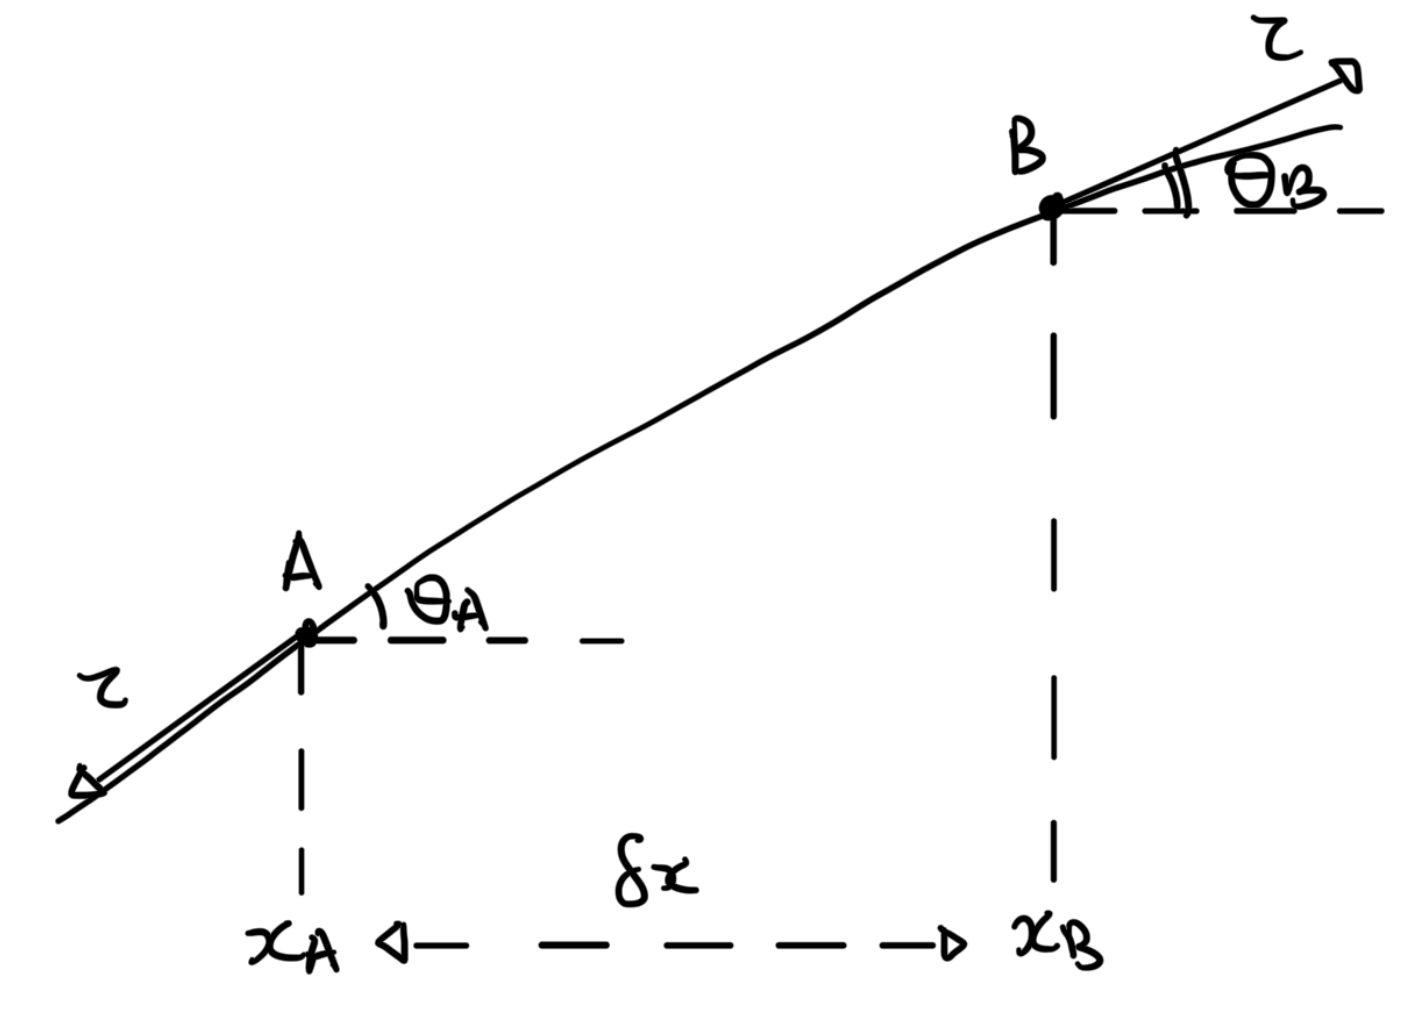
\includegraphics[width=0.5\textwidth]{fig/wave-equation-derivation.png}
    \caption{Derivation of the Wave Equation}
    \label{fig:wave-equation-derivation}%
\end{figure}

Consider a string under \emph{constant} tension \(\tau\), clanged at \(x = 0\) and \(x = L\). We allow the string to undergo small, transverse oscillations, so motion is constrained to be vertical each each point, and the displacement, \(y = y\pqty{x, y}\) obeys \(\abs{\pdv*{y}{x}} \ll 1\).

\small

Note that
\begin{equation}
    y\pqty{x}{t} = \int_{0}^{x} \pdv{y}{x} \pqty{s, t} \dd{s}
\end{equation}
and since \(y \pqty{0, t} = 0\), we have \(\abs{y} \ll L\).

\normalsize

Resolving horizontally, since there is no horizontal motion,
\begin{equation}
    \tau \cos\theta_B - \tan \cos \theta_A = 0
\end{equation}

This is consistent if we work up to \(\bigO\pqty{y_x^2}\). Using the fact that \(\tan\theta_A = y_x\pqty{x, t}\), and that \(\cos = \flatfrac{1}{\sqrt{\sec^2}}\), we have
\begin{subequations}
    \begin{align}
        \cos \theta_B - \cos \theta_A &= \frac{1}{\sqrt{1 + \pqty{\pdv*{y}{x}}^2_{B}}} - \frac{1}{\sqrt{1 + \pqty{\pdv*{y}{x}}^2_{B}}} \\
        &= \pdv{x} \bqty{\frac{1}{\sqrt{1 + \pqty{\pdv*{y}{x}}^2}}}_{x = \xi} \pqty{x_B - x_A} && \xi \in \oointv{x_A}{x_B} \\
        &= \bigO \pqty{\delta x \cdot y_x^2}
    \end{align}
\end{subequations}
so this is consistent.Mass of the string should be proportional to length, so
\begin{equation}
    \int_{A}^{B} \dd{s} = \int_{x_A}^{x_B} \sqrt{1 + \pqty{\pdv*{y}{x}}^2} \dd{x} = \delta x \bqty{1 + \bigO\pqty{y_x^2}}
\end{equation}
so it is reasonable to assume that the mass is \(\mu \delta x\), where \(\mu > 0\) is the string density.

Resolving vertically, by Newton's Second Law, we have
\begin{equation}
    \rightbar{\mu \delta x \pdv[2]{y}{t}}_{x = \frac{1}{2} \pqty{x_A + x_B}} = \tau \sin \theta_B - \tau \sin \theta_A.
\end{equation}

Using \(\sin = \cos \cdot \tan\), we have
\begin{subequations}
    \begin{align}
        \sin \theta_B - \sin \theta_A &= \frac{\pqty{\pdv*{y}{x}}_B}{\sqrt{1 + \pqty{\pdv*{y}{x}}^2_B}} - \frac{\pqty{\pdv*{y}{x}}_A}{\sqrt{1 + \pqty{\pdv*{y}{x}}^2_A}} \\
        &= \pdv{x} \bqty{\frac{y_x}{\sqrt{1 + y_x^2}}}_{x = \xi} \pqty{x_B - x_A} && \xi \in \oointv{x_A}{x_B} \\
        &= \bqty{y_xx + \bigO\pqty{y_x^2}} \delta x.
    \end{align}
\end{subequations}

So we have \(\mu \delta x \pdv*[2]{y}{t} = \tau \delta x \bqty{y_{xx} \pqty{\xi, t} + \bigO\pqty{y_x^2}}\), and taking \(\delta_x \to 0\) hence \(\xi \to x\), and hence this gives the \term{wave equation}
\begin{equation}
    \frac{1}{c^2} \pdv[2]{y}{t} = \pdv[2]{y}{x}, \quad c^2 = \frac{\tau}{\mu}.
\end{equation}
where \(c\) is known as the \term{wave speed}.

Here, we need to impose boundary conditions \(y\pqty{0, t} = y\pqty{L, t} = 0\) for all \(t \geq 0\), and initial conditions \(y\pqty{x, 0}\) (the \term{initial profile}) and \(\pdv*{y}{t} \pqty{x, 0}\) (the \term{initial velocity}) for \(0 \leq x \leq L\).

\subsubsection{Waves on a String}

The IBVP concerned in this section is given by
\begin{subequations}
    \begin{align}
        y_{tt} - c^2 y_{xx} = 0 &\qfor x \in \oointv{0}{L}, t > 0, \\
        y\pqty{0, t} = y\pqty{L, t} = 0 &\qfor t > 0, \\
        y\pqty{x, 0} = f\pqty{x} &\qfor x \in \oointv{0}{L}, \\
        y_t\pqty{x, 0} = g\pqty{x} &\qfor x \in \oointv{0}{L}.
    \end{align}
\end{subequations}

We attempt to solve the homogeneous part of the equation by separation of variables. Consider the ansatz \(y\pqty{x, t} = X\pqty{x} T\pqty{t}\), and substituting this into the PDE gives that for some \(\lambda \in \RR\), such that
\begin{subequations}
    \begin{align}
        X'' + \lambda X = 0 &\qfor 0 < x < L, \\
        X\pqty{0} = X\pqty{L} = 0 &\qfor x = 0, x = L, \\
        \ddot{T} + c^2 \lambda T = 0 &\qfor t > 0.
    \end{align}
\end{subequations}

Note that the first two equations are a Sturm--Liouville problem, and this solves to
\begin{equation}
    X_n\pqty{x} = \sin \pqty{\frac{n \pi x}{L}} \qfor \lambda_n = \pqty{\frac{n \pi}{L}}^2, \quad n = 1, 2, \ldots.
\end{equation}

Then the \(T\) equation reads
\begin{equation}
    \ddot{T} + \pqty{\frac{c n \pi}{L}}^2 T = 0,
\end{equation}
so
\begin{equation}
    T_n\pqty{t} = A_n \cos \pqty{\frac{c n \pi t}{L}} + B_n \sin \pqty{\frac{c n \pi t}{L}}.
\end{equation}

Therefore,
\begin{equation}
    y\pqty{x, t} = \sum_{n = 1}^{\infty} \sin \pqty{\frac{n \pi x}{L}} \bqty{A_n \cos \pqty{\frac{c n \pi t}{L}} + B_n \sin \pqty{\frac{c n \pi t}{L}}}.
\end{equation}

Initial conditions become
\begin{subequations}
    \begin{align}
        f\pqty{x} &= y\pqty{x, 0} = \sum_{n = 1}^{\infty} A_n \sin \pqty{\frac{n \pi x}{L}}, \\
        g\pqty{x} &= y_t\pqty{x, 0} = \sum_{n = 1}^{\infty} B_n \pqty{\frac{c n \pi}{L}} \sin \pqty{\frac{n \pi x}{L}}.
    \end{align}
\end{subequations}

Using the orthogonality of the sine functions \(\inner{X_n}{X_m} = \pqty{\flatfrac{L}{2}} \kronecker_{nm}\), we have
\begin{subequations}
    \begin{align}
        A_n &= \frac{2}{L} \int_{0}^{L} f\pqty{x} \sin \pqty{\frac{n \pi x}{L}} \dd{x}, \\
        B_n &= \frac{L}{c n \pi} \cdot \frac{2}{L} \int_{0}^{L} g\pqty{x} \sin \pqty{\frac{n \pi x}{L}} \dd{x}.
    \end{align}
\end{subequations}

\subsubsection{Waves on a Drum}

In hight dimensions, the wave equation becomes
\begin{equation}
    \frac{1}{c^2} \pdv[2]{\phi}{t} = \laplacian \phi \qfor \pqty{x, t} \in \Omega \times \oointv{0}{\plusinfty}.
\end{equation}

Then the IBVP becomes
\begin{subequations}
    \begin{align}
        \phi_{tt} - c^2 \laplacian \phi = 0 & \qfor \pqty{x, t} \in \Omega \times \oointv{0}{\plusinfty}, \\
        \phi\pqty{x, t} = 0 &\qfor \pqty{x, t} \in \partial \Omega \times \oointv{0}{\plusinfty}, \\
        \phi\pqty{x, 0} = f\pqty{x} &\qfor x \in \Omega, t = 0, \\
        \phi_t\pqty{x, 0} = g\pqty{x} &\qfor x \in \Omega, t = 0.
    \end{align}
\end{subequations}

We consider, in polar coordinates,
\begin{equation}
    \Omega = \set{\pqty/{r, \theta}}{r \in \cointv{0}{1}, \theta \in \cointv{0}{2 \pi}}.
\end{equation}

For simplicity, we assume \(f = f\pqty{r}\) and \(g = g\pqty{r}\), so we expect the solution to be of the form \(\phi = \phi\pqty{r, t}\). We solve the homogeneous problem with \(\phi = R\pqty{r} T\pqty{t}\), which gives
\begin{equation}
    \frac{\ddot{T}}{c^2 T} = \frac{\bqty{r R'}'}{rR}.
\end{equation}

So there is some \(\lambda \in \RR\), such that
\begin{subequations}
    \begin{align}
        - \dv{r} \bqty{r \dv{R}{r}} &= \lambda r R, \\
        R\pqty{1} &= 0 \\
        \ddot{T}+ c^2 \lambda T &= 0
    \end{align}
\end{subequations}

Note the radial equation is a Sturm--Liouville problem, and in particular, it is the Bessel equation of order \(m = 0\), so
\begin{equation}
    R_k \pqty{r} = J_0 \pqty{j_{0, k} r}, \quad \lambda_k = j_{0, k}^2, k = 1, 2, \ldots
\end{equation}
and the \(T\) equation now becomes
\begin{equation}
    \ddot{T} + \pqty{c j_{0, k}}^2 T = 0,
\end{equation}
whose solution is
\begin{equation}
    T_k\pqty{t} = A_k \cos \pqty{c j_{0, k} t} + B_k \sin \pqty{c j_{0, k} t}.
\end{equation}

Then the general solution is
\begin{equation}
    \phi\pqty{r, t} = \sum_{k = 1}^{\infty} J_0 \pqty{j_{0, k} r} \bqty{\begin{split}A_k \cos \pqty{c j_{0, k} t} \\ \quad+ B_k \sin \pqty{c j_{0, k} t}\end{split}}.
\end{equation}

\small

Recall that \begin{equation}
    \inner[w]{R_k}{R_l} = \frac{J_0' \pqty{j_{0, k}}^2}{2} \kronecker_{kl}.
\end{equation}

\normalsize

So we have
\begin{subequations}
    \begin{align}
        f\pqty{r} &= \sum_{k = 1}^{\infty} A_k J_0 \pqty{j_{0, k} r}, \\
        g\pqty{r} &= \sum_{k = 1}^{\infty} B_k j_{0, k} c J_0 \pqty{j_{0, k} r},
    \end{align}
\end{subequations}
and we may recover the coefficients
\begin{subequations}
    \begin{align}
        A_k &= \frac{2}{J_0' \pqty{j_{0, k}}^2} \int_{0}^{1} f\pqty{r} J_0 \pqty{j_{0, k} r} r \dd{r}, \\
        B_k &= \frac{1}{c j_{0, k}} \frac{2}{J_0' \pqty{j_{0, k}}^2} \int_{0}^{1} g\pqty{r} J_0 \pqty{j_{0, k} r} r \dd{r}.
    \end{align}
\end{subequations}